%% -*- coding:utf-8 -*-
\begin{figure}
\centering

\ifpdf
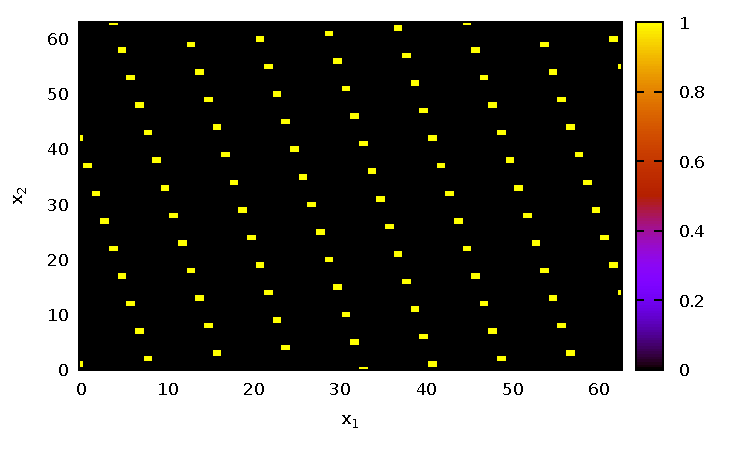
\includegraphics[angle=0]
{./part4/quantcomp/picellipticdiscretlog1.pdf}
\else
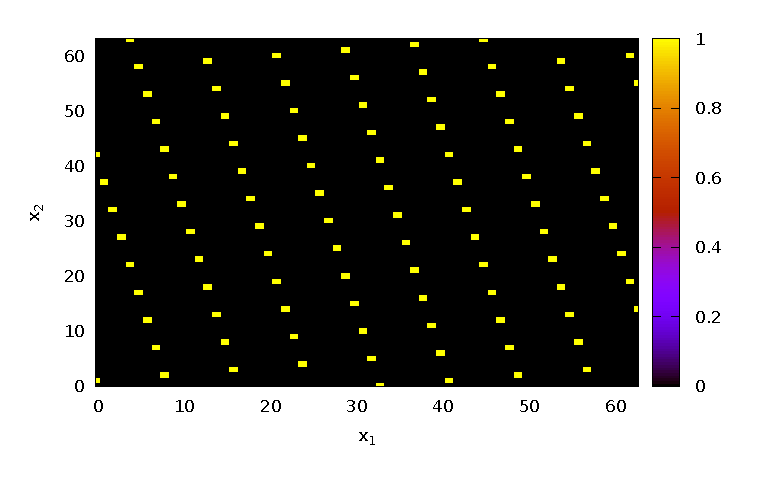
\includegraphics[angle=0]
{./part4/quantcomp/picellipticdiscretlog1.eps}
\fi

%\input ./part4/quantcomp/picdiscretlog2.tex

%% *Elliptic> c = Curve (-7) 10 97
%% *Elliptic> g = Point 96 93 c
%% *Elliptic> aa = Point 37 35 c
%% *Elliptic> filter (\(x1,x2) -> (1 .*. aa) .+. (2 .*. g) == g) [(x1,x2) | x1 <- [0..20], x2 <- [0..10]]
%% []
%% *Elliptic> filter (\(x1,x2) -> (x1 .*. aa) .+. (x2 .*. g) == g) [(x1,x2) | x1 <- [0..20], x2 <- [0..10]]
%% [(0,1),(7,7),(8,2),(15,8),(16,3)]

%% *Elliptic> (16 .*. aa) .+. (3 .*. g)
%% (96,93)


\caption{Graph of the function 
$f'(x_1, x_2)$ for $x_0 = 1$. Thus, points $x_1, x_2$ are shown
  corresponding to the relation $x_1 A + x_2 g = g$: 
  $x_1 (37, 35) + x_2 (96,93) = (96,93)$, for example
  $7 (37, 35) + 7 (96,93) = (96,93)$, $8 (37, 35) + 2 (96,93) =
  (96,93)$ or $16 (37, 35) + 3 (96,93) =
  (96,93)$. It is worth noting that the chosen pairs of points correspond
  to the condition \eqref{eq:part4:quantcomp:shorelliptic:fprime}, indeed
 we have $x \cdot 7 + 7 \equiv x \cdot 8 + 2 \mod 41$. 
 That is, if we subtract one from the other, we
 get an equation of the form $x \left(8-7\right) = - (2 - 7) = 5 \mod 41$.
 Or $x \equiv 5 \mod 41$} 
\label{fig:part4:quantcomp:dle1}
\end{figure}